\documentclass[twoside]{book}

% Packages required by doxygen
\usepackage{fixltx2e}
\usepackage{calc}
\usepackage{doxygen}
\usepackage[export]{adjustbox} % also loads graphicx
\usepackage{graphicx}
\usepackage[utf8]{inputenc}
\usepackage{makeidx}
\usepackage{multicol}
\usepackage{multirow}
\PassOptionsToPackage{warn}{textcomp}
\usepackage{textcomp}
\usepackage[nointegrals]{wasysym}
\usepackage[table]{xcolor}

% Font selection
\usepackage[T1]{fontenc}
\usepackage[scaled=.90]{helvet}
\usepackage{courier}
\usepackage{amssymb}
\usepackage{sectsty}
\renewcommand{\familydefault}{\sfdefault}
\allsectionsfont{%
  \fontseries{bc}\selectfont%
  \color{darkgray}%
}
\renewcommand{\DoxyLabelFont}{%
  \fontseries{bc}\selectfont%
  \color{darkgray}%
}
\newcommand{\+}{\discretionary{\mbox{\scriptsize$\hookleftarrow$}}{}{}}

% Page & text layout
\usepackage{geometry}
\geometry{%
  a4paper,%
  top=2.5cm,%
  bottom=2.5cm,%
  left=2.5cm,%
  right=2.5cm%
}
\tolerance=750
\hfuzz=15pt
\hbadness=750
\setlength{\emergencystretch}{15pt}
\setlength{\parindent}{0cm}
\setlength{\parskip}{3ex plus 2ex minus 2ex}
\makeatletter
\renewcommand{\paragraph}{%
  \@startsection{paragraph}{4}{0ex}{-1.0ex}{1.0ex}{%
    \normalfont\normalsize\bfseries\SS@parafont%
  }%
}
\renewcommand{\subparagraph}{%
  \@startsection{subparagraph}{5}{0ex}{-1.0ex}{1.0ex}{%
    \normalfont\normalsize\bfseries\SS@subparafont%
  }%
}
\makeatother

% Headers & footers
\usepackage{fancyhdr}
\pagestyle{fancyplain}
\fancyhead[LE]{\fancyplain{}{\bfseries\thepage}}
\fancyhead[CE]{\fancyplain{}{}}
\fancyhead[RE]{\fancyplain{}{\bfseries\leftmark}}
\fancyhead[LO]{\fancyplain{}{\bfseries\rightmark}}
\fancyhead[CO]{\fancyplain{}{}}
\fancyhead[RO]{\fancyplain{}{\bfseries\thepage}}
\fancyfoot[LE]{\fancyplain{}{}}
\fancyfoot[CE]{\fancyplain{}{}}
\fancyfoot[RE]{\fancyplain{}{\bfseries\scriptsize Generated by Doxygen }}
\fancyfoot[LO]{\fancyplain{}{\bfseries\scriptsize Generated by Doxygen }}
\fancyfoot[CO]{\fancyplain{}{}}
\fancyfoot[RO]{\fancyplain{}{}}
\renewcommand{\footrulewidth}{0.4pt}
\renewcommand{\chaptermark}[1]{%
  \markboth{#1}{}%
}
\renewcommand{\sectionmark}[1]{%
  \markright{\thesection\ #1}%
}

% Indices & bibliography
\usepackage{natbib}
\usepackage[titles]{tocloft}
\setcounter{tocdepth}{3}
\setcounter{secnumdepth}{5}
\makeindex

% Hyperlinks (required, but should be loaded last)
\usepackage{ifpdf}
\ifpdf
  \usepackage[pdftex,pagebackref=true]{hyperref}
\else
  \usepackage[ps2pdf,pagebackref=true]{hyperref}
\fi
\hypersetup{%
  colorlinks=true,%
  linkcolor=blue,%
  citecolor=blue,%
  unicode%
}

% Custom commands
\newcommand{\clearemptydoublepage}{%
  \newpage{\pagestyle{empty}\cleardoublepage}%
}

\usepackage{caption}
\captionsetup{labelsep=space,justification=centering,font={bf},singlelinecheck=off,skip=4pt,position=top}

%===== C O N T E N T S =====

\begin{document}

% Titlepage & ToC
\hypersetup{pageanchor=false,
             bookmarksnumbered=true,
             pdfencoding=unicode
            }
\pagenumbering{alph}
\begin{titlepage}
\vspace*{7cm}
\begin{center}%
{\Large cxx\+\_\+differentiation }\\
\vspace*{1cm}
{\large Generated by Doxygen 1.8.13}\\
\end{center}
\end{titlepage}
\clearemptydoublepage
\pagenumbering{roman}
\tableofcontents
\clearemptydoublepage
\pagenumbering{arabic}
\hypersetup{pageanchor=true}

%--- Begin generated contents ---
\chapter{The cxx\+\_\+differentiation library}
\label{index}\hypertarget{index}{}\hypertarget{index_intro}{}\section{Introduction and History}\label{index_intro}
The first significant library upgrade on the road to C++2011, \href{http://www.open-std.org/JTC1/SC22/WG21/docs/papers/2005/n1836.pdf}{\tt T\+R1}, included a set of 23 mathematical functions that significantly extended the standard transcendental functions inherited from C and declared in $<$cmath$>$.

Although most components from T\+R1 were eventually adopted for C++11 these math functions were left behind out of concern for implementability. The math functions were published as a separate international standard \href{http://www.open-std.org/JTC1/SC22/WG21/docs/papers/2010/n3060.pdf}{\tt IS 29124 -\/ Extensions to the C++ Library to Support Mathematical Special Functions}.

For C++17 these functions were incorporated into the main standard.\hypertarget{index_contents}{}\section{Contents}\label{index_contents}
The following functions are implemented in namespace {\ttfamily std\+:} 
\begin{DoxyItemize}
\item \hyperlink{group__tr29124__math__spec__func_ga87158c36cc84c104a3b23582829d8831}{assoc\+\_\+laguerre -\/ Associated Laguerre functions}
\item \hyperlink{group__tr29124__math__spec__func_ga9df2525c1155eb8539e85323f18361a3}{assoc\+\_\+legendre -\/ Associated Legendre functions}
\item \hyperlink{group__tr29124__math__spec__func_gaffed6cf5d5e3daf3e2c3a936bc0a33e7}{beta -\/ Beta functions}
\item \hyperlink{group__tr29124__math__spec__func_ga63f1e2ba4b94e170554d36882ee2be1d}{comp\+\_\+ellint\+\_\+1 -\/ Complete elliptic functions of the first kind}
\item \hyperlink{group__tr29124__math__spec__func_gacd0057c6937200dc296c98d7e53f5112}{comp\+\_\+ellint\+\_\+2 -\/ Complete elliptic functions of the second kind}
\item \hyperlink{group__tr29124__math__spec__func_gae3abb5ca753f218c4c17fe7dc9feabc4}{comp\+\_\+ellint\+\_\+3 -\/ Complete elliptic functions of the third kind}
\item \hyperlink{group__tr29124__math__spec__func_gac2ce366244694be909cd13bf8e1b439c}{cyl\+\_\+bessel\+\_\+i -\/ Regular modified cylindrical Bessel functions}
\item \hyperlink{group__tr29124__math__spec__func_ga968904e6095c70b275858f8e684403fb}{cyl\+\_\+bessel\+\_\+j -\/ Cylindrical Bessel functions of the first kind}
\item \hyperlink{group__tr29124__math__spec__func_ga3cd72edf8e8ef6f225d9c4a067f9423e}{cyl\+\_\+bessel\+\_\+k -\/ Irregular modified cylindrical Bessel functions}
\item \hyperlink{group__tr29124__math__spec__func_gaa5720700a9d1c33f30b53c6b30ec3260}{cyl\+\_\+neumann -\/ Cylindrical Neumann functions or Cylindrical Bessel functions of the second kind}
\item \hyperlink{group__tr29124__math__spec__func_ga8be90518215c6209679785e5444ee0af}{ellint\+\_\+1 -\/ Incomplete elliptic functions of the first kind}
\item \hyperlink{group__tr29124__math__spec__func_ga6db0d1043cad03894edb7def7b70bc39}{ellint\+\_\+2 -\/ Incomplete elliptic functions of the second kind}
\item \hyperlink{group__tr29124__math__spec__func_ga3af251108b5384ca1f27350e47c8108e}{ellint\+\_\+3 -\/ Incomplete elliptic functions of the third kind}
\item \hyperlink{group__tr29124__math__spec__func_gac6d12da409bbd0e41dd1f7cdb3317252}{expint -\/ The exponential integral}
\item \hyperlink{group__tr29124__math__spec__func_gaded38c372f2977d30b613bd55426f132}{hermite -\/ Hermite polynomials}
\item \hyperlink{group__tr29124__math__spec__func_gaf1927ca6432351e3a7af47e158e63862}{laguerre -\/ Laguerre functions}
\item \hyperlink{group__tr29124__math__spec__func_ga327bb7686d2e63d85e8c6b1b42b3b29e}{legendre -\/ Legendre polynomials}
\item \hyperlink{group__tr29124__math__spec__func_ga57bb10396587a75e909d3c6e47dadf20}{riemann\+\_\+zeta -\/ The Riemann zeta function}
\item \hyperlink{group__tr29124__math__spec__func_ga52331d03089052b53d96c776c62e4997}{sph\+\_\+bessel -\/ Spherical Bessel functions}
\item \hyperlink{group__tr29124__math__spec__func_ga5b33a8e403bfa3c6df370e163310d66c}{sph\+\_\+legendre -\/ Spherical Legendre functions}
\item \hyperlink{group__tr29124__math__spec__func_gae8528a53bb38d600c6c517a7ec10039e}{sph\+\_\+neumann -\/ Spherical Neumann functions}
\end{DoxyItemize}

The hypergeometric functions were stricken from the T\+R29124 and C++17 versions of this math library because of implementation concerns. However, since they were in the T\+R1 version and since they are popular we kept them as an extension in namespace {\ttfamily \hyperlink{namespace____gnu__cxx}{\+\_\+\+\_\+gnu\+\_\+cxx}\+:} 
\begin{DoxyItemize}
\item \hyperlink{group__gnu__math__spec__func_ga5e71f453c84b767792dc26ffda96f8fb}{conf\+\_\+hyperg -\/ Confluent hypergeometric functions}
\item \hyperlink{group__gnu__math__spec__func_ga40de7f02b2adfe6a883a85698720d7fd}{hyperg -\/ Hypergeometric functions}
\end{DoxyItemize}

In addition a large number of new functions are added as extensions\+:
\begin{DoxyItemize}
\item \hyperlink{group__gnu__math__spec__func_ga53243cdb83abeb008fa90d8a098768af}{airy\+\_\+ai -\/ Airy functions of the first kind}
\item \hyperlink{group__gnu__math__spec__func_ga812ca309bff1b0ae2bbe1183a0bc47d5}{airy\+\_\+bi -\/ Airy functions of the second kind}
\item \hyperlink{group__gnu__math__spec__func_ga2934ccfb8bbd5877efd369a3ecd9ac4d}{bincoef -\/ Binomial coefficients}
\item \hyperlink{group__gnu__math__spec__func_gacf63ebbc67ea21d569cf510ed0da95fd}{bose\+\_\+einstein -\/ Bose-\/\+Einstein integrals}
\item \hyperlink{group__gnu__math__spec__func_gae35c0bc63248e3bcdb9b490477975eb4}{chebyshev\+\_\+t -\/ Chebyshev polynomials of the first kind}
\item \hyperlink{group__gnu__math__spec__func_gaea7ea830fe6be79ca84fba1bb94691a4}{chebyshev\+\_\+u -\/ Chebyshev polynomials of the second kind}
\item \hyperlink{group__gnu__math__spec__func_ga674e3d97204a74620eb0d408873aefb9}{chebyshev\+\_\+v -\/ Chebyshev polynomials of the third kind}
\item \hyperlink{group__gnu__math__spec__func_ga55ebf3cda76302bc6e0f173fc1c1425e}{chebyshev\+\_\+w -\/ Chebyshev polynomials of the fourth kind}
\item \hyperlink{group__gnu__math__spec__func_ga7959ce3dea7f8d98b1dfee5715303f1c}{clausen -\/ Clausen integrals}
\item \hyperlink{group__gnu__math__spec__func_gabbdae75b253a0b19e8ae3d42c14f6be3}{clausen\+\_\+c -\/ Clausen cosine integrals}
\item \hyperlink{group__gnu__math__spec__func_ga3ed0e444799410cda76ccbc62181ce0c}{clausen\+\_\+s -\/ Clausen sine integrals}
\item \hyperlink{group__gnu__math__spec__func_ga2c6b6c5a44ea00f0aed05c02f1072c31}{comp\+\_\+ellint\+\_\+d -\/ Incomplete Legendre D elliptic integral}
\item \hyperlink{group__gnu__math__spec__func_gab923b5a9e67469a5145d7bfcb20b3396}{conf\+\_\+hyperg\+\_\+lim -\/ Confluent hypergeometric limit functions}
\item \hyperlink{group__gnu__math__spec__func_ga05f183d57b1726136ba9795ba1b158c5}{cos\+\_\+pi -\/ Reperiodized cosine function.}
\item \hyperlink{group__gnu__math__spec__func_ga633224563637e80a4cda93863a693ad6}{cosh\+\_\+pi -\/ Reperiodized hyperbolic cosine function.}
\item \hyperlink{group__gnu__math__spec__func_ga901c23871fded7d4467a864fe06bbf07}{coshint -\/ Hyperbolic cosine integral}
\item \hyperlink{group__gnu__math__spec__func_ga06eed76a045a73ad72fcf4ad00b05f96}{cosint -\/ Cosine integral}
\item \hyperlink{group__gnu__math__spec__func_gafa5ad1cfd4cc30caaeb06bdab71e600b}{cyl\+\_\+hankel\+\_\+1 -\/ Cylindrical Hankel functions of the first kind}
\item \hyperlink{group__gnu__math__spec__func_ga6c1d2d390e547ded9e0f4cc46395d90c}{cyl\+\_\+hankel\+\_\+2 -\/ Cylindrical Hankel functions of the second kind}
\item \hyperlink{group__gnu__math__spec__func_ga0623ddcbfdce696781e19648fde6f33a}{dawson -\/ Dawson integrals}
\item \hyperlink{group__gnu__math__spec__func_ga7a95a3cb9a53aca2a1ff9752ce9d5e3c}{dilog -\/ Dilogarithm functions}
\item \hyperlink{group__gnu__math__spec__func_ga87466a2d429a2815d794acc21c882b08}{dirichlet\+\_\+beta -\/ Dirichlet beta function}
\item \hyperlink{group__gnu__math__spec__func_gae46e26e4107675d285c79a2d6202e6c7}{dirichlet\+\_\+eta -\/ Dirichlet beta function}
\item \hyperlink{group__gnu__math__spec__func_ga06842a81bdcabf9c62252dde992d42ee}{dirichlet\+\_\+lambda -\/ Dirichlet lambda function}
\item \hyperlink{group__gnu__math__spec__func_ga08c31a5dd1686a7633b46f923c47af46}{double\+\_\+factorial -\/ }
\item \hyperlink{group__gnu__math__spec__func_ga71785ba6bad83f009cb2dc4d2d574194}{ellint\+\_\+d -\/ Legendre D elliptic integrals}
\item \hyperlink{group__gnu__math__spec__func_ga21b90daf6c8d705b052304905809d2db}{ellint\+\_\+rc -\/ Carlson elliptic functions R\+\_\+C}
\item \hyperlink{group__gnu__math__spec__func_ga6467a19028332392df825e232a97139f}{ellint\+\_\+rd -\/ Carlson elliptic functions R\+\_\+D}
\item \hyperlink{group__gnu__math__spec__func_ga9242fbc43bd340e0def2a6f15b755c1c}{ellint\+\_\+rf -\/ Carlson elliptic functions R\+\_\+F}
\item \hyperlink{group__gnu__math__spec__func_gab525116e1b311da90e2745366ac314eb}{ellint\+\_\+rg -\/ Carlson elliptic functions R\+\_\+G}
\item \hyperlink{group__gnu__math__spec__func_gaf9a96979913713963c5f4edeba8c7f5a}{ellint\+\_\+rj -\/ Carlson elliptic functions R\+\_\+J}
\item \hyperlink{group__gnu__math__spec__func_ga7bfb34f8b5c0ed7c72040f9cb7034bba}{ellnome -\/ Elliptic nome}
\item \hyperlink{group__gnu__math__spec__func_ga2cfc699129ceac9cfed87c61e6dc0e08}{expint -\/ Exponential integrals}
\item \hyperlink{group__gnu__math__spec__func_ga48bc268969bfc03eaeaf4bfd457bb25c}{factorial -\/ Factorials}
\item \hyperlink{group__gnu__math__spec__func_ga47dd583a4f3a19f797a5e074e357ba36}{fermi\+\_\+dirac -\/ Fermi-\/\+Dirac integrals}
\item \hyperlink{group__gnu__math__spec__func_gab6a34ce43bad4e8181ad9c40aebb9ada}{fresnel\+\_\+c -\/ Fresnel cosine integrals}
\item \hyperlink{group__gnu__math__spec__func_gaaf6e2b182d0abde6fde72c0b8b9f959c}{fresnel\+\_\+s -\/ Fresnel sine integrals}
\item \hyperlink{group__gnu__math__spec__func_ga793df814fb4e1b60e926ead0be14cc87}{gegenbauer -\/ Gegenbauer polynomials}
\item \hyperlink{group__gnu__math__spec__func_gab73b2a75a662785fa102926dca3be59f}{heuman\+\_\+lambda -\/ Heuman lambda functions}
\item \hyperlink{group__gnu__math__spec__func_ga19b3014d94dd102c59a5c7776474be41}{hurwitz\+\_\+zeta -\/ Hurwitz zeta functions}
\item \hyperlink{group__gnu__math__spec__func_gae9a18423e325171ca0c61b411258fa65}{ibeta -\/ Regularized incomplete beta functions}
\item \hyperlink{group__gnu__math__spec__func_ga3dea9ec3774ee5db50276597bbfb0afa}{jacobi -\/ Jacobi polynomials}
\item \hyperlink{group__gnu__math__spec__func_ga5e39ec723669e132e27980dfdf766c19}{jacobi\+\_\+sn -\/ Jacobi sine amplitude functions}
\item \hyperlink{group__gnu__math__spec__func_ga51512996a910489b4554daa7507a48f1}{jacobi\+\_\+cn -\/ Jacobi cosine amplitude functions}
\item \hyperlink{group__gnu__math__spec__func_ga4c2e5ff17abaab5217d4dbcbfd7366d8}{jacobi\+\_\+dn -\/ Jacobi delta amplitude functions}
\item \hyperlink{group__gnu__math__spec__func_gafe1fc209cfe90ceee3b42e077a922045}{jacobi\+\_\+zeta -\/ Jacobi zeta functions}
\item \hyperlink{group__gnu__math__spec__func_gab6a2243313b6286cbd466c96fc7f69ed}{lbincoef -\/ Log binomial coefficients}
\item \hyperlink{group__gnu__math__spec__func_ga31ca8e7a5b1f5c883e727ed9c053edd8}{ldouble\+\_\+factorial -\/ Log double factorials}
\item \hyperlink{group__gnu__math__spec__func_ga4ad68133a4ff354cb99e4d3608ce6e4d}{legendre\+\_\+q -\/ Legendre functions of the second kind}
\item \hyperlink{group__gnu__math__spec__func_gaee28cc03db944a3e02fd10542016cfa8}{lfactorial -\/ Log factorials}
\item \hyperlink{group__gnu__math__spec__func_gaf70747491390b1bfc27b93ff4be6376e}{lgamma -\/ Log gamma for complex arguments}
\item \hyperlink{group__gnu__math__spec__func_ga4975d412b8e15f499a4da7b4e3f535c6}{lpochhammer\+\_\+lower -\/ Log lower Pochhammer functions}
\item \hyperlink{group__gnu__math__spec__func_ga68c4a9e8b38757a21ac54c55fe4e8dda}{lpochhammer -\/ Log upper Pochhammer functions}
\item \hyperlink{group__gnu__math__spec__func_gaa6ca4f2127c6c2101dc360673304cc2c}{owens\+\_\+t -\/ Owens T functions}
\item \hyperlink{group__gnu__math__spec__func_gaa78927de2c62e6c63f4b3506f5e1a8f6}{pgamma -\/ Regularized lower incomplete gamma functions}
\item \hyperlink{group__gnu__math__spec__func_ga306d65eeea07613a777f506ffadac509}{pochhammer\+\_\+lower -\/ Lower Pochhammer functions}
\item \hyperlink{group__gnu__math__spec__func_ga77878c3e202c7ec3d857c3fbf661001e}{pochhammer -\/ Upper Pochhammer functions}
\item \hyperlink{group__gnu__math__spec__func_gaae7574990cdbb6a637d39c2c036928c0}{psi -\/ Psi or digamma function}
\item \hyperlink{group__gnu__math__spec__func_ga3ef7aeaa55f9e7b02f02d1d605a716a6}{qgamma -\/ Regularized upper incomplete gamma functions}
\item \hyperlink{group__gnu__math__spec__func_gac44ad9bda660a21a6b297d313f0ecf48}{radpoly -\/ Radial polynomials}
\item \hyperlink{group__gnu__math__spec__func_gabafa26d8a2e592a0e080beae71ccbb7e}{sinhc -\/ Hyperbolic sinus cardinal function}
\item \hyperlink{group__gnu__math__spec__func_ga56bea42a4701761e82567f7100d9ca5e}{sinhc\+\_\+pi -\/ }
\item \hyperlink{group__gnu__math__spec__func_ga6a11b9d949ab86f9fd170dcf0d3b1251}{sinc -\/ Normalized sinus cardinal function}
\item \hyperlink{group__gnu__math__spec__func_ga8041c24b528475bcf8a4178e484652a3}{sincos -\/ Sine + cosine function}
\item \hyperlink{group__gnu__math__spec__func_ga3152cfc9d5fa04fbe61781b45b3d4c04}{sincos\+\_\+pi -\/ Reperiodized sine + cosine function}
\item \hyperlink{group__gnu__math__spec__func_ga8fcd01a56e0c16d7568026c0bb4312eb}{sin\+\_\+pi -\/ Reperiodized sine function.}
\item \hyperlink{group__gnu__math__spec__func_gab004f7356231c96ae819d72e5d75b8dd}{sinh\+\_\+pi -\/ Reperiodized hyperbolic sine function.}
\item \hyperlink{group__gnu__math__spec__func_ga3dbc3831c1bd9f2a8be05496db9375a0}{sinc\+\_\+pi -\/ Sinus cardinal function}
\item \hyperlink{group__gnu__math__spec__func_ga203079a2b70127f16a8c434ea55d4e06}{sinhint -\/ Hyperbolic sine integral}
\item \hyperlink{group__gnu__math__spec__func_gaa588265d28710d36c7c4efa7d4f44ca4}{sinint -\/ Sine integral}
\item \hyperlink{group__gnu__math__spec__func_gad168511a86d4d25db99e2b08d5da038b}{sph\+\_\+bessel\+\_\+i -\/ Spherical regular modified Bessel functions}
\item \hyperlink{group__gnu__math__spec__func_ga9ad96c43b15e2c53d2f1b743e2eaa90f}{sph\+\_\+bessel\+\_\+k -\/ Spherical iregular modified Bessel functions}
\item \hyperlink{group__gnu__math__spec__func_ga04c91059810f366e3366fadef9084be7}{sph\+\_\+hankel\+\_\+1 -\/ Spherical Hankel functions of the first kind}
\item \hyperlink{group__gnu__math__spec__func_gafb5debe7f7db9e9e456c065acf738f64}{sph\+\_\+hankel\+\_\+2 -\/ Spherical Hankel functions of the first kind}
\item \hyperlink{group__gnu__math__spec__func_gadca3d25c4f7eed15099d8f80681d4055}{sph\+\_\+harmonic -\/ Spherical}
\item \hyperlink{group__gnu__math__spec__func_ga5029c1e804c1c9b28949b5ef00237c08}{tan\+\_\+pi -\/ Reperiodized tangent function.}
\item \hyperlink{group__gnu__math__spec__func_ga5f0c92cb16210a8d087327ff2c048115}{tanh\+\_\+pi -\/ Reperiodized hyperbolic tangent function.}
\item \hyperlink{group__gnu__math__spec__func_ga6133351c7602e917fd08d62d897e57d0}{tgamma -\/ Gamma for complex arguments}
\item \hyperlink{group__gnu__math__spec__func_ga6133351c7602e917fd08d62d897e57d0}{tgamma -\/ Upper incomplete gamma functions}
\item \hyperlink{group__gnu__math__spec__func_ga973fba718e906a5179d954c56b991c8d}{tgamma\+\_\+lower -\/ Lower incomplete gamma functions}
\item \hyperlink{group__gnu__math__spec__func_gac122af3ffd2e5536fdf021afce79b7d4}{theta\+\_\+1 -\/ Exponential theta function 1}
\item \hyperlink{group__gnu__math__spec__func_gacec36dc316e561bbaa371c60c06e52f7}{theta\+\_\+2 -\/ Exponential theta function 2}
\item \hyperlink{group__gnu__math__spec__func_ga34e5d79e6ba8b8b104e690fc1ebc7fd6}{theta\+\_\+3 -\/ Exponential theta function 3}
\item \hyperlink{group__gnu__math__spec__func_ga25e72f2b50b53d168f8fa653b1a0d012}{theta\+\_\+4 -\/ Exponential theta function 4}
\item \hyperlink{group__gnu__math__spec__func_ga5df3bb50b78cd1bc676763dbf9e64929}{zernike -\/ Zernike polynomials}
\end{DoxyItemize}\hypertarget{index_general}{}\section{General Features}\label{index_general}
\hypertarget{index_promotion}{}\subsection{Argument Promotion}\label{index_promotion}
The arguments suppled to the non-\/suffixed functions will be promoted according to the following rules\+:
\begin{DoxyEnumerate}
\item If any argument intended to be floating point is given an integral value That integral value is promoted to double.
\item All floating point arguments are promoted up to the largest floating point precision among them.
\end{DoxyEnumerate}\hypertarget{index_NaN}{}\subsection{Na\+N Arguments}\label{index_NaN}
If any of the floating point arguments supplied to these functions is invalid or NaN (std\+::numeric\+\_\+limits$<$\+Tp$>$\+::quiet\+\_\+\+NaN), the value NaN is returned.\hypertarget{index_impl}{}\section{Implementation}\label{index_impl}
We strive to implement the underlying math with type generic algorithms to the greatest extent possible. In practice, the functions are thin wrappers that dispatch to function templates. Type dependence is controlled with std\+::numeric\+\_\+limits and functions thereof.

We don\textquotesingle{}t promote {\ttfamily float} to {\ttfamily double} or {\ttfamily double} to {\ttfamily long double} reflexively. The goal is for {\ttfamily float} functions to operate more quickly, at the cost of {\ttfamily float} accuracy and possibly a smaller domain of validity. Similaryly, {\ttfamily long double} should give you more dynamic range and slightly more pecision than {\ttfamily double} on many systems.\hypertarget{index_testing}{}\section{Testing}\label{index_testing}
These functions have been tested against equivalent implementations from the \href{http://www.gnu.org/software/gsl}{\tt Gnu Scientific Library, G\+SL} and $<$a href="\href{http://www.boost.org/doc/libs/1_60_0/libs/math/doc/html/index.html}{\tt http\+://www.\+boost.\+org/doc/libs/1\+\_\+60\+\_\+0/libs/math/doc/html/index.\+html}$>$Boost and the ratio \[ \frac{|f - f_{test}|}{|f_{test}|} \] is generally found to be within 10$^\wedge$-\/15 for 64-\/bit double on linux-\/x86\+\_\+64 systems over most of the ranges of validity.

\begin{DoxyRefDesc}{Todo}
\item[\hyperlink{todo__todo000001}{Todo}]Provide accuracy comparisons on a per-\/function basis for a small number of targets.\end{DoxyRefDesc}
\hypertarget{index_bibliography}{}\section{General Bibliography}\label{index_bibliography}
\begin{DoxySeeAlso}{See also}
Abramowitz and Stegun\+: Handbook of Mathematical Functions, with Formulas, Graphs, and Mathematical Tables Edited by Milton Abramowitz and Irene A. Stegun, National Bureau of Standards Applied Mathematics Series -\/ 55 Issued June 1964, Tenth Printing, December 1972, with corrections Electronic versions of A\&S abound including both pdf and navigable html. 

for example \href{http://people.math.sfu.ca/~cbm/aands/}{\tt http\+://people.\+math.\+sfu.\+ca/$\sim$cbm/aands/}

The old A\&S has been redone as the N\+I\+ST Digital Library of Mathematical Functions\+: \href{http://dlmf.nist.gov/}{\tt http\+://dlmf.\+nist.\+gov/} This version is far more navigable and includes more recent work.

An Atlas of Functions\+: with Equator, the Atlas Function Calculator 2nd Edition, by Oldham, Keith B., Myland, Jan, Spanier, Jerome

Asymptotics and Special Functions by Frank W. J. Olver, Academic Press, 1974

Numerical Recipes in C, The Art of Scientific Computing, by William H. Press, Second Ed., Saul A. Teukolsky, William T. Vetterling, and Brian P. Flannery, Cambridge University Press, 1992

The Special Functions and Their Approximations\+: Volumes 1 and 2, by Yudell L. Luke, Academic Press, 1969 
\end{DoxySeeAlso}

\chapter{Class Index}
\section{Class List}
Here are the classes, structs, unions and interfaces with brief descriptions\+:\begin{DoxyCompactList}
\item\contentsline{section}{\hyperlink{struct____gnu__cxx_1_1____airy__t}{\+\_\+\+\_\+gnu\+\_\+cxx\+::\+\_\+\+\_\+airy\+\_\+t$<$ \+\_\+\+Tx, \+\_\+\+Tp $>$} }{\pageref{struct____gnu__cxx_1_1____airy__t}}{}
\item\contentsline{section}{\hyperlink{struct____gnu__cxx_1_1____cyl__bessel__t}{\+\_\+\+\_\+gnu\+\_\+cxx\+::\+\_\+\+\_\+cyl\+\_\+bessel\+\_\+t$<$ \+\_\+\+Tnu, \+\_\+\+Tx, \+\_\+\+Tp $>$} }{\pageref{struct____gnu__cxx_1_1____cyl__bessel__t}}{}
\item\contentsline{section}{\hyperlink{struct____gnu__cxx_1_1____cyl__hankel__t}{\+\_\+\+\_\+gnu\+\_\+cxx\+::\+\_\+\+\_\+cyl\+\_\+hankel\+\_\+t$<$ \+\_\+\+Tnu, \+\_\+\+Tx, \+\_\+\+Tp $>$} }{\pageref{struct____gnu__cxx_1_1____cyl__hankel__t}}{}
\item\contentsline{section}{\hyperlink{struct____gnu__cxx_1_1____cyl__mod__bessel__t}{\+\_\+\+\_\+gnu\+\_\+cxx\+::\+\_\+\+\_\+cyl\+\_\+mod\+\_\+bessel\+\_\+t$<$ \+\_\+\+Tnu, \+\_\+\+Tx, \+\_\+\+Tp $>$} }{\pageref{struct____gnu__cxx_1_1____cyl__mod__bessel__t}}{}
\item\contentsline{section}{\hyperlink{struct____gnu__cxx_1_1____fock__airy__t}{\+\_\+\+\_\+gnu\+\_\+cxx\+::\+\_\+\+\_\+fock\+\_\+airy\+\_\+t$<$ \+\_\+\+Tx, \+\_\+\+Tp $>$} }{\pageref{struct____gnu__cxx_1_1____fock__airy__t}}{}
\item\contentsline{section}{\hyperlink{struct____gnu__cxx_1_1____fp__is__integer__t}{\+\_\+\+\_\+gnu\+\_\+cxx\+::\+\_\+\+\_\+fp\+\_\+is\+\_\+integer\+\_\+t} }{\pageref{struct____gnu__cxx_1_1____fp__is__integer__t}}{}
\item\contentsline{section}{\hyperlink{struct____gnu__cxx_1_1____gamma__inc__t}{\+\_\+\+\_\+gnu\+\_\+cxx\+::\+\_\+\+\_\+gamma\+\_\+inc\+\_\+t$<$ \+\_\+\+Tp $>$} }{\pageref{struct____gnu__cxx_1_1____gamma__inc__t}}{}
\item\contentsline{section}{\hyperlink{struct____gnu__cxx_1_1____gamma__temme__t}{\+\_\+\+\_\+gnu\+\_\+cxx\+::\+\_\+\+\_\+gamma\+\_\+temme\+\_\+t$<$ \+\_\+\+Tp $>$} \\*A structure for the gamma functions required by the Temme series expansions of $ N_\nu(x) $ and $ K_\nu(x) $. \[ \Gamma_1 = \frac{1}{2\mu} \left[\frac{1}{\Gamma(1 - \mu)} - \frac{1}{\Gamma(1 + \mu)}\right] \] and \[ \Gamma_2 = \frac{1}{2} \left[\frac{1}{\Gamma(1 - \mu)} + \frac{1}{\Gamma(1 + \mu)}\right] \] where $ -1/2 <= \mu <= 1/2 $ is $ \mu = \nu - N $ and $ N $. is the nearest integer to $ \nu $. The values of $ \Gamma(1 + \mu) $ and $ \Gamma(1 - \mu) $ are returned as well }{\pageref{struct____gnu__cxx_1_1____gamma__temme__t}}{}
\item\contentsline{section}{\hyperlink{struct____gnu__cxx_1_1____jacobi__t}{\+\_\+\+\_\+gnu\+\_\+cxx\+::\+\_\+\+\_\+jacobi\+\_\+t$<$ \+\_\+\+Tp $>$} }{\pageref{struct____gnu__cxx_1_1____jacobi__t}}{}
\item\contentsline{section}{\hyperlink{struct____gnu__cxx_1_1____lgamma__t}{\+\_\+\+\_\+gnu\+\_\+cxx\+::\+\_\+\+\_\+lgamma\+\_\+t$<$ \+\_\+\+Tp $>$} }{\pageref{struct____gnu__cxx_1_1____lgamma__t}}{}
\item\contentsline{section}{\hyperlink{struct____gnu__cxx_1_1____pqgamma__t}{\+\_\+\+\_\+gnu\+\_\+cxx\+::\+\_\+\+\_\+pqgamma\+\_\+t$<$ \+\_\+\+Tp $>$} }{\pageref{struct____gnu__cxx_1_1____pqgamma__t}}{}
\item\contentsline{section}{\hyperlink{struct____gnu__cxx_1_1____quadrature__point__t}{\+\_\+\+\_\+gnu\+\_\+cxx\+::\+\_\+\+\_\+quadrature\+\_\+point\+\_\+t$<$ \+\_\+\+Tp $>$} }{\pageref{struct____gnu__cxx_1_1____quadrature__point__t}}{}
\item\contentsline{section}{\hyperlink{struct____gnu__cxx_1_1____sincos__t}{\+\_\+\+\_\+gnu\+\_\+cxx\+::\+\_\+\+\_\+sincos\+\_\+t$<$ \+\_\+\+Tp $>$} }{\pageref{struct____gnu__cxx_1_1____sincos__t}}{}
\item\contentsline{section}{\hyperlink{struct____gnu__cxx_1_1____sph__bessel__t}{\+\_\+\+\_\+gnu\+\_\+cxx\+::\+\_\+\+\_\+sph\+\_\+bessel\+\_\+t$<$ \+\_\+\+Tn, \+\_\+\+Tx, \+\_\+\+Tp $>$} }{\pageref{struct____gnu__cxx_1_1____sph__bessel__t}}{}
\item\contentsline{section}{\hyperlink{struct____gnu__cxx_1_1____sph__hankel__t}{\+\_\+\+\_\+gnu\+\_\+cxx\+::\+\_\+\+\_\+sph\+\_\+hankel\+\_\+t$<$ \+\_\+\+Tn, \+\_\+\+Tx, \+\_\+\+Tp $>$} }{\pageref{struct____gnu__cxx_1_1____sph__hankel__t}}{}
\item\contentsline{section}{\hyperlink{struct____gnu__cxx_1_1____sph__mod__bessel__t}{\+\_\+\+\_\+gnu\+\_\+cxx\+::\+\_\+\+\_\+sph\+\_\+mod\+\_\+bessel\+\_\+t$<$ \+\_\+\+Tn, \+\_\+\+Tx, \+\_\+\+Tp $>$} }{\pageref{struct____gnu__cxx_1_1____sph__mod__bessel__t}}{}
\item\contentsline{section}{\hyperlink{structstd_1_1____detail_1_1____gamma__lanczos__data}{std\+::\+\_\+\+\_\+detail\+::\+\_\+\+\_\+gamma\+\_\+lanczos\+\_\+data$<$ \+\_\+\+Tp $>$} }{\pageref{structstd_1_1____detail_1_1____gamma__lanczos__data}}{}
\item\contentsline{section}{\hyperlink{structstd_1_1____detail_1_1____gamma__lanczos__data_3_01double_01_4}{std\+::\+\_\+\+\_\+detail\+::\+\_\+\+\_\+gamma\+\_\+lanczos\+\_\+data$<$ double $>$} }{\pageref{structstd_1_1____detail_1_1____gamma__lanczos__data_3_01double_01_4}}{}
\item\contentsline{section}{\hyperlink{structstd_1_1____detail_1_1____gamma__lanczos__data_3_01float_01_4}{std\+::\+\_\+\+\_\+detail\+::\+\_\+\+\_\+gamma\+\_\+lanczos\+\_\+data$<$ float $>$} }{\pageref{structstd_1_1____detail_1_1____gamma__lanczos__data_3_01float_01_4}}{}
\item\contentsline{section}{\hyperlink{structstd_1_1____detail_1_1____gamma__lanczos__data_3_01long_01double_01_4}{std\+::\+\_\+\+\_\+detail\+::\+\_\+\+\_\+gamma\+\_\+lanczos\+\_\+data$<$ long double $>$} }{\pageref{structstd_1_1____detail_1_1____gamma__lanczos__data_3_01long_01double_01_4}}{}
\item\contentsline{section}{\hyperlink{structstd_1_1____detail_1_1____gamma__spouge__data}{std\+::\+\_\+\+\_\+detail\+::\+\_\+\+\_\+gamma\+\_\+spouge\+\_\+data$<$ \+\_\+\+Tp $>$} }{\pageref{structstd_1_1____detail_1_1____gamma__spouge__data}}{}
\item\contentsline{section}{\hyperlink{structstd_1_1____detail_1_1____gamma__spouge__data_3_01double_01_4}{std\+::\+\_\+\+\_\+detail\+::\+\_\+\+\_\+gamma\+\_\+spouge\+\_\+data$<$ double $>$} }{\pageref{structstd_1_1____detail_1_1____gamma__spouge__data_3_01double_01_4}}{}
\item\contentsline{section}{\hyperlink{structstd_1_1____detail_1_1____gamma__spouge__data_3_01float_01_4}{std\+::\+\_\+\+\_\+detail\+::\+\_\+\+\_\+gamma\+\_\+spouge\+\_\+data$<$ float $>$} }{\pageref{structstd_1_1____detail_1_1____gamma__spouge__data_3_01float_01_4}}{}
\item\contentsline{section}{\hyperlink{structstd_1_1____detail_1_1____gamma__spouge__data_3_01long_01double_01_4}{std\+::\+\_\+\+\_\+detail\+::\+\_\+\+\_\+gamma\+\_\+spouge\+\_\+data$<$ long double $>$} }{\pageref{structstd_1_1____detail_1_1____gamma__spouge__data_3_01long_01double_01_4}}{}
\item\contentsline{section}{\hyperlink{classstd_1_1____detail_1_1__Airy}{std\+::\+\_\+\+\_\+detail\+::\+\_\+\+Airy$<$ \+\_\+\+Tp $>$} }{\pageref{classstd_1_1____detail_1_1__Airy}}{}
\item\contentsline{section}{\hyperlink{classstd_1_1____detail_1_1__Airy__asymp}{std\+::\+\_\+\+\_\+detail\+::\+\_\+\+Airy\+\_\+asymp$<$ \+\_\+\+Tp $>$} }{\pageref{classstd_1_1____detail_1_1__Airy__asymp}}{}
\item\contentsline{section}{\hyperlink{structstd_1_1____detail_1_1__Airy__asymp__data}{std\+::\+\_\+\+\_\+detail\+::\+\_\+\+Airy\+\_\+asymp\+\_\+data$<$ \+\_\+\+Tp $>$} }{\pageref{structstd_1_1____detail_1_1__Airy__asymp__data}}{}
\item\contentsline{section}{\hyperlink{structstd_1_1____detail_1_1__Airy__asymp__data_3_01double_01_4}{std\+::\+\_\+\+\_\+detail\+::\+\_\+\+Airy\+\_\+asymp\+\_\+data$<$ double $>$} }{\pageref{structstd_1_1____detail_1_1__Airy__asymp__data_3_01double_01_4}}{}
\item\contentsline{section}{\hyperlink{structstd_1_1____detail_1_1__Airy__asymp__data_3_01float_01_4}{std\+::\+\_\+\+\_\+detail\+::\+\_\+\+Airy\+\_\+asymp\+\_\+data$<$ float $>$} }{\pageref{structstd_1_1____detail_1_1__Airy__asymp__data_3_01float_01_4}}{}
\item\contentsline{section}{\hyperlink{structstd_1_1____detail_1_1__Airy__asymp__data_3_01long_01double_01_4}{std\+::\+\_\+\+\_\+detail\+::\+\_\+\+Airy\+\_\+asymp\+\_\+data$<$ long double $>$} }{\pageref{structstd_1_1____detail_1_1__Airy__asymp__data_3_01long_01double_01_4}}{}
\item\contentsline{section}{\hyperlink{classstd_1_1____detail_1_1__Airy__asymp__series}{std\+::\+\_\+\+\_\+detail\+::\+\_\+\+Airy\+\_\+asymp\+\_\+series$<$ \+\_\+\+Sum $>$} }{\pageref{classstd_1_1____detail_1_1__Airy__asymp__series}}{}
\item\contentsline{section}{\hyperlink{structstd_1_1____detail_1_1__Airy__default__radii}{std\+::\+\_\+\+\_\+detail\+::\+\_\+\+Airy\+\_\+default\+\_\+radii$<$ \+\_\+\+Tp $>$} }{\pageref{structstd_1_1____detail_1_1__Airy__default__radii}}{}
\item\contentsline{section}{\hyperlink{structstd_1_1____detail_1_1__Airy__default__radii_3_01double_01_4}{std\+::\+\_\+\+\_\+detail\+::\+\_\+\+Airy\+\_\+default\+\_\+radii$<$ double $>$} }{\pageref{structstd_1_1____detail_1_1__Airy__default__radii_3_01double_01_4}}{}
\item\contentsline{section}{\hyperlink{structstd_1_1____detail_1_1__Airy__default__radii_3_01float_01_4}{std\+::\+\_\+\+\_\+detail\+::\+\_\+\+Airy\+\_\+default\+\_\+radii$<$ float $>$} }{\pageref{structstd_1_1____detail_1_1__Airy__default__radii_3_01float_01_4}}{}
\item\contentsline{section}{\hyperlink{structstd_1_1____detail_1_1__Airy__default__radii_3_01long_01double_01_4}{std\+::\+\_\+\+\_\+detail\+::\+\_\+\+Airy\+\_\+default\+\_\+radii$<$ long double $>$} }{\pageref{structstd_1_1____detail_1_1__Airy__default__radii_3_01long_01double_01_4}}{}
\item\contentsline{section}{\hyperlink{classstd_1_1____detail_1_1__Airy__series}{std\+::\+\_\+\+\_\+detail\+::\+\_\+\+Airy\+\_\+series$<$ \+\_\+\+Tp $>$} }{\pageref{classstd_1_1____detail_1_1__Airy__series}}{}
\item\contentsline{section}{\hyperlink{structstd_1_1____detail_1_1__AiryAuxilliaryState}{std\+::\+\_\+\+\_\+detail\+::\+\_\+\+Airy\+Auxilliary\+State$<$ \+\_\+\+Tp $>$} }{\pageref{structstd_1_1____detail_1_1__AiryAuxilliaryState}}{}
\item\contentsline{section}{\hyperlink{structstd_1_1____detail_1_1__AiryState}{std\+::\+\_\+\+\_\+detail\+::\+\_\+\+Airy\+State$<$ \+\_\+\+Tp $>$} }{\pageref{structstd_1_1____detail_1_1__AiryState}}{}
\item\contentsline{section}{\hyperlink{structstd_1_1____detail_1_1__Factorial__table}{std\+::\+\_\+\+\_\+detail\+::\+\_\+\+Factorial\+\_\+table$<$ \+\_\+\+Tp $>$} }{\pageref{structstd_1_1____detail_1_1__Factorial__table}}{}
\end{DoxyCompactList}

\chapter{File Index}
\section{File List}
Here is a list of all files with brief descriptions\+:\begin{DoxyCompactList}
\item\contentsline{section}{bits/\hyperlink{sf__airy_8tcc}{sf\+\_\+airy.\+tcc} }{\pageref{sf__airy_8tcc}}{}
\item\contentsline{section}{bits/\hyperlink{sf__bernoulli_8tcc}{sf\+\_\+bernoulli.\+tcc} }{\pageref{sf__bernoulli_8tcc}}{}
\item\contentsline{section}{bits/\hyperlink{sf__bessel_8tcc}{sf\+\_\+bessel.\+tcc} }{\pageref{sf__bessel_8tcc}}{}
\item\contentsline{section}{bits/\hyperlink{sf__beta_8tcc}{sf\+\_\+beta.\+tcc} }{\pageref{sf__beta_8tcc}}{}
\item\contentsline{section}{bits/\hyperlink{sf__cardinal_8tcc}{sf\+\_\+cardinal.\+tcc} }{\pageref{sf__cardinal_8tcc}}{}
\item\contentsline{section}{bits/\hyperlink{sf__chebyshev_8tcc}{sf\+\_\+chebyshev.\+tcc} }{\pageref{sf__chebyshev_8tcc}}{}
\item\contentsline{section}{bits/\hyperlink{sf__coulomb_8tcc}{sf\+\_\+coulomb.\+tcc} }{\pageref{sf__coulomb_8tcc}}{}
\item\contentsline{section}{bits/\hyperlink{sf__dawson_8tcc}{sf\+\_\+dawson.\+tcc} }{\pageref{sf__dawson_8tcc}}{}
\item\contentsline{section}{bits/\hyperlink{sf__distributions_8tcc}{sf\+\_\+distributions.\+tcc} }{\pageref{sf__distributions_8tcc}}{}
\item\contentsline{section}{bits/\hyperlink{sf__ellint_8tcc}{sf\+\_\+ellint.\+tcc} }{\pageref{sf__ellint_8tcc}}{}
\item\contentsline{section}{bits/\hyperlink{sf__euler_8tcc}{sf\+\_\+euler.\+tcc} }{\pageref{sf__euler_8tcc}}{}
\item\contentsline{section}{bits/\hyperlink{sf__expint_8tcc}{sf\+\_\+expint.\+tcc} }{\pageref{sf__expint_8tcc}}{}
\item\contentsline{section}{bits/\hyperlink{sf__fresnel_8tcc}{sf\+\_\+fresnel.\+tcc} }{\pageref{sf__fresnel_8tcc}}{}
\item\contentsline{section}{bits/\hyperlink{sf__gamma_8tcc}{sf\+\_\+gamma.\+tcc} }{\pageref{sf__gamma_8tcc}}{}
\item\contentsline{section}{bits/\hyperlink{sf__gegenbauer_8tcc}{sf\+\_\+gegenbauer.\+tcc} }{\pageref{sf__gegenbauer_8tcc}}{}
\item\contentsline{section}{bits/\hyperlink{sf__hankel_8tcc}{sf\+\_\+hankel.\+tcc} }{\pageref{sf__hankel_8tcc}}{}
\item\contentsline{section}{bits/\hyperlink{sf__hermite_8tcc}{sf\+\_\+hermite.\+tcc} }{\pageref{sf__hermite_8tcc}}{}
\item\contentsline{section}{bits/\hyperlink{sf__hyperg_8tcc}{sf\+\_\+hyperg.\+tcc} }{\pageref{sf__hyperg_8tcc}}{}
\item\contentsline{section}{bits/\hyperlink{sf__hypint_8tcc}{sf\+\_\+hypint.\+tcc} }{\pageref{sf__hypint_8tcc}}{}
\item\contentsline{section}{bits/\hyperlink{sf__jacobi_8tcc}{sf\+\_\+jacobi.\+tcc} }{\pageref{sf__jacobi_8tcc}}{}
\item\contentsline{section}{bits/\hyperlink{sf__laguerre_8tcc}{sf\+\_\+laguerre.\+tcc} }{\pageref{sf__laguerre_8tcc}}{}
\item\contentsline{section}{bits/\hyperlink{sf__legendre_8tcc}{sf\+\_\+legendre.\+tcc} }{\pageref{sf__legendre_8tcc}}{}
\item\contentsline{section}{bits/\hyperlink{sf__mod__bessel_8tcc}{sf\+\_\+mod\+\_\+bessel.\+tcc} }{\pageref{sf__mod__bessel_8tcc}}{}
\item\contentsline{section}{bits/\hyperlink{sf__owens__t_8tcc}{sf\+\_\+owens\+\_\+t.\+tcc} }{\pageref{sf__owens__t_8tcc}}{}
\item\contentsline{section}{bits/\hyperlink{sf__polylog_8tcc}{sf\+\_\+polylog.\+tcc} }{\pageref{sf__polylog_8tcc}}{}
\item\contentsline{section}{bits/\hyperlink{sf__stirling_8tcc}{sf\+\_\+stirling.\+tcc} }{\pageref{sf__stirling_8tcc}}{}
\item\contentsline{section}{bits/\hyperlink{sf__theta_8tcc}{sf\+\_\+theta.\+tcc} }{\pageref{sf__theta_8tcc}}{}
\item\contentsline{section}{bits/\hyperlink{sf__trig_8tcc}{sf\+\_\+trig.\+tcc} }{\pageref{sf__trig_8tcc}}{}
\item\contentsline{section}{bits/\hyperlink{sf__trigint_8tcc}{sf\+\_\+trigint.\+tcc} }{\pageref{sf__trigint_8tcc}}{}
\item\contentsline{section}{bits/\hyperlink{sf__zeta_8tcc}{sf\+\_\+zeta.\+tcc} }{\pageref{sf__zeta_8tcc}}{}
\item\contentsline{section}{bits/\hyperlink{specfun_8h}{specfun.\+h} }{\pageref{specfun_8h}}{}
\item\contentsline{section}{bits/\hyperlink{specfun__state_8h}{specfun\+\_\+state.\+h} }{\pageref{specfun__state_8h}}{}
\item\contentsline{section}{ext/\hyperlink{math__util_8h}{math\+\_\+util.\+h} }{\pageref{math__util_8h}}{}
\end{DoxyCompactList}

\chapter{Class Documentation}
\hypertarget{structderivative__t}{}\section{derivative\+\_\+t$<$ \+\_\+\+Tp $>$ Struct Template Reference}
\label{structderivative__t}\index{derivative\+\_\+t$<$ \+\_\+\+Tp $>$@{derivative\+\_\+t$<$ \+\_\+\+Tp $>$}}


{\ttfamily \#include $<$derivative.\+h$>$}

\subsection*{Public Attributes}
\begin{DoxyCompactItemize}
\item 
\mbox{\Hypertarget{structderivative__t_a80c4b0dfdc6e2dcc8a9802d60dbb73ee}\label{structderivative__t_a80c4b0dfdc6e2dcc8a9802d60dbb73ee}} 
\+\_\+\+Tp \hyperlink{structderivative__t_a80c4b0dfdc6e2dcc8a9802d60dbb73ee}{value}
\begin{DoxyCompactList}\small\item\em The value of the derivative. \end{DoxyCompactList}\item 
\mbox{\Hypertarget{structderivative__t_ac9a4904da8901950967bdc5e6b1cc012}\label{structderivative__t_ac9a4904da8901950967bdc5e6b1cc012}} 
\+\_\+\+Tp \hyperlink{structderivative__t_ac9a4904da8901950967bdc5e6b1cc012}{error\+\_\+trunc}
\begin{DoxyCompactList}\small\item\em The absolute value of the truncation error. \end{DoxyCompactList}\item 
\mbox{\Hypertarget{structderivative__t_a423825c0784d7156c5e71075eb6c2103}\label{structderivative__t_a423825c0784d7156c5e71075eb6c2103}} 
\+\_\+\+Tp \hyperlink{structderivative__t_a423825c0784d7156c5e71075eb6c2103}{error\+\_\+round}
\begin{DoxyCompactList}\small\item\em The absolute value of the rounding error. \end{DoxyCompactList}\end{DoxyCompactItemize}


\subsection{Detailed Description}
\subsubsection*{template$<$typename \+\_\+\+Tp$>$\newline
struct derivative\+\_\+t$<$ \+\_\+\+Tp $>$}

A struct conaining the results of a numerical differentiation. 

The documentation for this struct was generated from the following file\+:\begin{DoxyCompactItemize}
\item 
include/ext/derivative.\+h\end{DoxyCompactItemize}

\chapter{File Documentation}
\hypertarget{differentiation_8h}{}\section{include/ext/differentiation.h File Reference}
\label{differentiation_8h}\index{include/ext/differentiation.\+h@{include/ext/differentiation.\+h}}
{\ttfamily \#include $<$ext/differentiation.\+tcc$>$}\newline
Include dependency graph for differentiation.\+h\+:\nopagebreak
\begin{figure}[H]
\begin{center}
\leavevmode
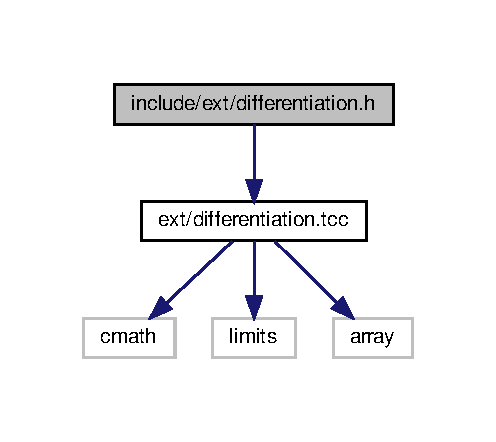
\includegraphics[width=238pt]{differentiation_8h__incl}
\end{center}
\end{figure}
\subsection*{Classes}
\begin{DoxyCompactItemize}
\item 
struct \hyperlink{structderivative__t}{derivative\+\_\+t$<$ \+\_\+\+Tp $>$}
\end{DoxyCompactItemize}
\subsection*{Functions}
\begin{DoxyCompactItemize}
\item 
{\footnotesize template$<$typename \+\_\+\+Func , typename \+\_\+\+Tp $>$ }\\\hyperlink{structderivative__t}{derivative\+\_\+t}$<$ \+\_\+\+Tp $>$ \hyperlink{differentiation_8h_aef32000eba6743a6066fdd345ab72f17}{derivative\+\_\+central} (\+\_\+\+Func \+\_\+\+\_\+func, \+\_\+\+Tp \+\_\+\+\_\+x, \+\_\+\+Tp \+\_\+\+\_\+h)
\item 
{\footnotesize template$<$typename \+\_\+\+Func , typename \+\_\+\+Tp $>$ }\\\hyperlink{structderivative__t}{derivative\+\_\+t}$<$ \+\_\+\+Tp $>$ \hyperlink{differentiation_8h_ac1cc760446a1455c0e97fe098dde2bc7}{derivative\+\_\+forward} (\+\_\+\+Func \+\_\+\+\_\+func, \+\_\+\+Tp \+\_\+\+\_\+x, \+\_\+\+Tp \+\_\+\+\_\+h)
\item 
{\footnotesize template$<$typename \+\_\+\+Func , typename \+\_\+\+Tp $>$ }\\\hyperlink{structderivative__t}{derivative\+\_\+t}$<$ \+\_\+\+Tp $>$ \hyperlink{differentiation_8h_abf178afb597679c287a7f8269d89a394}{derivative\+\_\+backward} (\+\_\+\+Func \+\_\+\+\_\+func, \+\_\+\+Tp \+\_\+\+\_\+x, \+\_\+\+Tp \+\_\+\+\_\+h)
\item 
{\footnotesize template$<$typename \+\_\+\+Func , typename \+\_\+\+Tp $>$ }\\\hyperlink{structderivative__t}{derivative\+\_\+t}$<$ \+\_\+\+Tp $>$ \hyperlink{differentiation_8h_a3e9da1abac5e2d4a10e0eeca1812590d}{derivative\+\_\+ridder} (\+\_\+\+Func \+\_\+\+\_\+func, \+\_\+\+Tp \+\_\+\+\_\+x, \+\_\+\+Tp \+\_\+\+\_\+h)
\end{DoxyCompactItemize}


\subsection{Detailed Description}
This file contains the declarations and the inline implementations of the differentiation data structures and routines. 

\subsection{Function Documentation}
\mbox{\Hypertarget{differentiation_8h_abf178afb597679c287a7f8269d89a394}\label{differentiation_8h_abf178afb597679c287a7f8269d89a394}} 
\index{differentiation.\+h@{differentiation.\+h}!derivative\+\_\+backward@{derivative\+\_\+backward}}
\index{derivative\+\_\+backward@{derivative\+\_\+backward}!differentiation.\+h@{differentiation.\+h}}
\subsubsection{\texorpdfstring{derivative\+\_\+backward()}{derivative\_backward()}}
{\footnotesize\ttfamily template$<$typename \+\_\+\+Func , typename \+\_\+\+Tp $>$ \\
\hyperlink{structderivative__t}{derivative\+\_\+t}$<$\+\_\+\+Tp$>$ derivative\+\_\+backward (\begin{DoxyParamCaption}\item[{\+\_\+\+Func}]{\+\_\+\+\_\+func,  }\item[{\+\_\+\+Tp}]{\+\_\+\+\_\+x,  }\item[{\+\_\+\+Tp}]{\+\_\+\+\_\+h }\end{DoxyParamCaption})\hspace{0.3cm}{\ttfamily [inline]}}

Compute the derivative using the 4-\/point rule (x -\/ h/4, x -\/ h/2, x -\/ 3h/4, x -\/ h).

Compute the error using the difference between the 4-\/point and the 2-\/point rule (x -\/ h/2, x -\/ h).

i.\+e. run the forward differentiator with negative stepsize.


\begin{DoxyTemplParams}{Template Parameters}
{\em \+\_\+\+Func} & A function type callable with a numeric type and returning the same. \\
\hline
{\em \+\_\+\+Tp} & The foating point type of the argument and stepsize.\\
\hline
\end{DoxyTemplParams}

\begin{DoxyParams}{Parameters}
{\em \+\_\+\+\_\+func} & The function to be differentated. \\
\hline
{\em \+\_\+\+\_\+x} & The location at which the derivative is required. \\
\hline
{\em \+\_\+\+\_\+h} & The stepsize. \\
\hline
\end{DoxyParams}
\mbox{\Hypertarget{differentiation_8h_aef32000eba6743a6066fdd345ab72f17}\label{differentiation_8h_aef32000eba6743a6066fdd345ab72f17}} 
\index{differentiation.\+h@{differentiation.\+h}!derivative\+\_\+central@{derivative\+\_\+central}}
\index{derivative\+\_\+central@{derivative\+\_\+central}!differentiation.\+h@{differentiation.\+h}}
\subsubsection{\texorpdfstring{derivative\+\_\+central()}{derivative\_central()}}
{\footnotesize\ttfamily template$<$typename \+\_\+\+Func , typename \+\_\+\+Tp $>$ \\
\hyperlink{structderivative__t}{derivative\+\_\+t}$<$\+\_\+\+Tp$>$ derivative\+\_\+central (\begin{DoxyParamCaption}\item[{\+\_\+\+Func}]{\+\_\+\+\_\+func,  }\item[{\+\_\+\+Tp}]{\+\_\+\+\_\+x,  }\item[{\+\_\+\+Tp}]{\+\_\+\+\_\+h }\end{DoxyParamCaption})}

Compute the derivative using the 5-\/point rule (x-\/h, x-\/h/2, x, x+h/2, x+h). Note that the central point is not used.

Compute the error using the difference between the 5-\/point and the 3-\/point rule (x-\/h, x, x+h). Again the central point is not used.


\begin{DoxyTemplParams}{Template Parameters}
{\em \+\_\+\+Func} & A function type callable with a numeric type and returning the same. \\
\hline
{\em \+\_\+\+Tp} & The foating point type of the argument and stepsize.\\
\hline
\end{DoxyTemplParams}

\begin{DoxyParams}{Parameters}
{\em \+\_\+\+\_\+func} & The function to be differentated. \\
\hline
{\em \+\_\+\+\_\+x} & The location at which the derivative is required. \\
\hline
{\em \+\_\+\+\_\+h} & The stepsize. \\
\hline
\end{DoxyParams}
\mbox{\Hypertarget{differentiation_8h_ac1cc760446a1455c0e97fe098dde2bc7}\label{differentiation_8h_ac1cc760446a1455c0e97fe098dde2bc7}} 
\index{differentiation.\+h@{differentiation.\+h}!derivative\+\_\+forward@{derivative\+\_\+forward}}
\index{derivative\+\_\+forward@{derivative\+\_\+forward}!differentiation.\+h@{differentiation.\+h}}
\subsubsection{\texorpdfstring{derivative\+\_\+forward()}{derivative\_forward()}}
{\footnotesize\ttfamily template$<$typename \+\_\+\+Func , typename \+\_\+\+Tp $>$ \\
\hyperlink{structderivative__t}{derivative\+\_\+t}$<$\+\_\+\+Tp$>$ derivative\+\_\+forward (\begin{DoxyParamCaption}\item[{\+\_\+\+Func}]{\+\_\+\+\_\+func,  }\item[{\+\_\+\+Tp}]{\+\_\+\+\_\+x,  }\item[{\+\_\+\+Tp}]{\+\_\+\+\_\+h }\end{DoxyParamCaption})}

Compute the derivative using the 4-\/point rule (x + h/4, x + h/2, x + 3h/4, x + h).

Compute the error using the difference between the 4-\/point and the 2-\/point rule (x + h/2, x+h).


\begin{DoxyTemplParams}{Template Parameters}
{\em \+\_\+\+Func} & A function type callable with a numeric type and returning the same. \\
\hline
{\em \+\_\+\+Tp} & The foating point type of the argument and stepsize.\\
\hline
\end{DoxyTemplParams}

\begin{DoxyParams}{Parameters}
{\em \+\_\+\+\_\+func} & The function to be differentated. \\
\hline
{\em \+\_\+\+\_\+x} & The location at which the derivative is required. \\
\hline
{\em \+\_\+\+\_\+h} & The stepsize. \\
\hline
\end{DoxyParams}
\mbox{\Hypertarget{differentiation_8h_a3e9da1abac5e2d4a10e0eeca1812590d}\label{differentiation_8h_a3e9da1abac5e2d4a10e0eeca1812590d}} 
\index{differentiation.\+h@{differentiation.\+h}!derivative\+\_\+ridder@{derivative\+\_\+ridder}}
\index{derivative\+\_\+ridder@{derivative\+\_\+ridder}!differentiation.\+h@{differentiation.\+h}}
\subsubsection{\texorpdfstring{derivative\+\_\+ridder()}{derivative\_ridder()}}
{\footnotesize\ttfamily template$<$typename \+\_\+\+Func , typename \+\_\+\+Tp $>$ \\
\hyperlink{structderivative__t}{derivative\+\_\+t}$<$\+\_\+\+Tp$>$ derivative\+\_\+ridder (\begin{DoxyParamCaption}\item[{\+\_\+\+Func}]{\+\_\+\+\_\+func,  }\item[{\+\_\+\+Tp}]{\+\_\+\+\_\+x,  }\item[{\+\_\+\+Tp}]{\+\_\+\+\_\+h }\end{DoxyParamCaption})}

Compute the derivative of a function func at a point x by Ridder\textquotesingle{}s method of polynomial extrapolation.

The value h is input as an estimated stepsize; it should not be small but rather it should be an interval over which the function changes substantially.


\begin{DoxyTemplParams}{Template Parameters}
{\em \+\_\+\+Func} & A function type callable with a numeric type and returning the same. \\
\hline
{\em \+\_\+\+Tp} & The foating point type of the argument and stepsize.\\
\hline
\end{DoxyTemplParams}

\begin{DoxyParams}{Parameters}
{\em \+\_\+\+\_\+func} & The function to be differentated. \\
\hline
{\em \+\_\+\+\_\+x} & The location at which the derivative is required. \\
\hline
{\em \+\_\+\+\_\+h} & The initial stepsize. \\
\hline
\end{DoxyParams}

\hypertarget{differentiation_8tcc}{}\doxysection{include/emsr/differentiation.tcc File Reference}
\label{differentiation_8tcc}\index{include/emsr/differentiation.tcc@{include/emsr/differentiation.tcc}}
{\ttfamily \#include $<$cmath$>$}\newline
{\ttfamily \#include $<$limits$>$}\newline
{\ttfamily \#include $<$array$>$}\newline
{\ttfamily \#include $<$complex$>$}\newline
Include dependency graph for differentiation.\+tcc\+:
\nopagebreak
\begin{figure}[H]
\begin{center}
\leavevmode
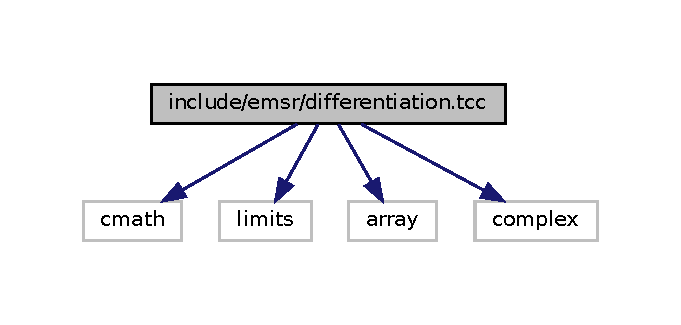
\includegraphics[width=327pt]{differentiation_8tcc__incl}
\end{center}
\end{figure}
\doxysubsection*{Macros}
\begin{DoxyCompactItemize}
\item 
\#define \mbox{\hyperlink{differentiation_8tcc_aba2d54628bdc01e26d172ef294c3e0f8}{DIFFERENTIATION\+\_\+\+TCC}}~1
\end{DoxyCompactItemize}
\doxysubsection*{Functions}
\begin{DoxyCompactItemize}
\item 
{\footnotesize template$<$typename Func , typename Tp $>$ }\\\mbox{\hyperlink{structderivative__t}{derivative\+\_\+t}}$<$ Tp $>$ \mbox{\hyperlink{differentiation_8tcc_a6ab76f5ee2c247487dd77d4a1ac0d023}{derivative\+\_\+central}} (Func func, Tp x, Tp h)
\item 
{\footnotesize template$<$typename Func , typename Tp $>$ }\\\mbox{\hyperlink{structderivative__t}{derivative\+\_\+t}}$<$ Tp $>$ \mbox{\hyperlink{differentiation_8tcc_a2fd096a92e6b977a98fd7d16a04dc8b4}{derivative\+\_\+forward}} (Func func, Tp x, Tp h)
\item 
{\footnotesize template$<$typename Func , typename Tp $>$ }\\\mbox{\hyperlink{structderivative__t}{derivative\+\_\+t}}$<$ Tp $>$ \mbox{\hyperlink{differentiation_8tcc_ad773ecd26f4d7a6754acecdc833639a2}{derivative\+\_\+ridder}} (Func func, Tp x, Tp h)
\item 
{\footnotesize template$<$typename Func , typename Tp $>$ }\\\mbox{\hyperlink{structderivative__t}{derivative\+\_\+t}}$<$ Tp $>$ \mbox{\hyperlink{differentiation_8tcc_a03f1970cde537ff0aef96f4b9af8a06e}{derivative\+\_\+automatic}} (Func func, Tp x, Tp)
\end{DoxyCompactItemize}


\doxysubsection{Detailed Description}
This file contains the outline implementation of the differentiation routines. 

\doxysubsection{Macro Definition Documentation}
\mbox{\Hypertarget{differentiation_8tcc_aba2d54628bdc01e26d172ef294c3e0f8}\label{differentiation_8tcc_aba2d54628bdc01e26d172ef294c3e0f8}} 
\index{differentiation.tcc@{differentiation.tcc}!DIFFERENTIATION\_TCC@{DIFFERENTIATION\_TCC}}
\index{DIFFERENTIATION\_TCC@{DIFFERENTIATION\_TCC}!differentiation.tcc@{differentiation.tcc}}
\doxysubsubsection{\texorpdfstring{DIFFERENTIATION\_TCC}{DIFFERENTIATION\_TCC}}
{\footnotesize\ttfamily \#define DIFFERENTIATION\+\_\+\+TCC~1}



\doxysubsection{Function Documentation}
\mbox{\Hypertarget{differentiation_8tcc_a03f1970cde537ff0aef96f4b9af8a06e}\label{differentiation_8tcc_a03f1970cde537ff0aef96f4b9af8a06e}} 
\index{differentiation.tcc@{differentiation.tcc}!derivative\_automatic@{derivative\_automatic}}
\index{derivative\_automatic@{derivative\_automatic}!differentiation.tcc@{differentiation.tcc}}
\doxysubsubsection{\texorpdfstring{derivative\_automatic()}{derivative\_automatic()}}
{\footnotesize\ttfamily template$<$typename Func , typename Tp $>$ \\
\mbox{\hyperlink{structderivative__t}{derivative\+\_\+t}}$<$Tp$>$ derivative\+\_\+automatic (\begin{DoxyParamCaption}\item[{Func}]{func,  }\item[{Tp}]{x,  }\item[{Tp}]{ }\end{DoxyParamCaption})}

Compute the derivative of a function func at a point x by automatic differentiation\+: \[ f\textnormal{\textquotesingle}(x) = Im[f(x + i\epsilon)] / \epsilon \] This routine ignores the input stepsize and uses machine epsilon.

If your function has complex overloads and works at least very near the real axis this is a very accurate routine.


\begin{DoxyTemplParams}{Template Parameters}
{\em Func} & A function type callable with a numeric type and returning the same. \\
\hline
{\em Tp} & The foating point type of the argument and stepsize.\\
\hline
\end{DoxyTemplParams}

\begin{DoxyParams}{Parameters}
{\em func} & The function to be differentated. \\
\hline
{\em x} & The (real) location at which the derivative is required. \\
\hline
{\em h} & The initial stepsize. \\
\hline
\end{DoxyParams}
\mbox{\Hypertarget{differentiation_8tcc_a6ab76f5ee2c247487dd77d4a1ac0d023}\label{differentiation_8tcc_a6ab76f5ee2c247487dd77d4a1ac0d023}} 
\index{differentiation.tcc@{differentiation.tcc}!derivative\_central@{derivative\_central}}
\index{derivative\_central@{derivative\_central}!differentiation.tcc@{differentiation.tcc}}
\doxysubsubsection{\texorpdfstring{derivative\_central()}{derivative\_central()}}
{\footnotesize\ttfamily template$<$typename Func , typename Tp $>$ \\
\mbox{\hyperlink{structderivative__t}{derivative\+\_\+t}}$<$Tp$>$ derivative\+\_\+central (\begin{DoxyParamCaption}\item[{Func}]{func,  }\item[{Tp}]{x,  }\item[{Tp}]{h }\end{DoxyParamCaption})}

Compute the derivative using the 5-\/point rule (x-\/h, x-\/h/2, x, x+h/2, x+h). Note that the central point is not used. \[ f\textnormal{\textquotesingle}_3(x) = \frac{f(x + h) - f(x - h)}{2h} \] \[ f\textnormal{\textquotesingle}_5(x) = \frac{4}{3}\frac{f(x + h/2) - f(x - h/2)}{2h} - \frac{1}{3}f\textnormal{\textquotesingle}_3(x) \]

Compute the error using the difference between the 5-\/point and the 3-\/point rule (x-\/h, x, x+h). Again the central point is not used.


\begin{DoxyTemplParams}{Template Parameters}
{\em Func} & A function type callable with a numeric type and returning the same. \\
\hline
{\em Tp} & The foating point type of the argument and stepsize.\\
\hline
\end{DoxyTemplParams}

\begin{DoxyParams}{Parameters}
{\em func} & The function to be differentated. \\
\hline
{\em x} & The location at which the derivative is required. \\
\hline
{\em h} & The stepsize. \\
\hline
\end{DoxyParams}
\mbox{\Hypertarget{differentiation_8tcc_a2fd096a92e6b977a98fd7d16a04dc8b4}\label{differentiation_8tcc_a2fd096a92e6b977a98fd7d16a04dc8b4}} 
\index{differentiation.tcc@{differentiation.tcc}!derivative\_forward@{derivative\_forward}}
\index{derivative\_forward@{derivative\_forward}!differentiation.tcc@{differentiation.tcc}}
\doxysubsubsection{\texorpdfstring{derivative\_forward()}{derivative\_forward()}}
{\footnotesize\ttfamily template$<$typename Func , typename Tp $>$ \\
\mbox{\hyperlink{structderivative__t}{derivative\+\_\+t}}$<$Tp$>$ derivative\+\_\+forward (\begin{DoxyParamCaption}\item[{Func}]{func,  }\item[{Tp}]{x,  }\item[{Tp}]{h }\end{DoxyParamCaption})}

Compute the derivative using the 4-\/point rule (x + h/4, x + h/2, x + 3h/4, x + h). \[ f\textnormal{\textquotesingle}_2(x) = \frac{f(x + h) - f(x + h/2)}{h/2} \] \[ f\textnormal{\textquotesingle}_4(x) = \frac{22(f(x + h) - f(x + 3h/4)) - 62(f(x + 3h/4) - f(x + h/2)) + 52(f(x + h/2 - f(x + h/4))}{3h} \]

Compute the error using the difference between the 4-\/point and the 2-\/point rule (x + h/2, x+h).


\begin{DoxyTemplParams}{Template Parameters}
{\em Func} & A function type callable with a numeric type and returning the same. \\
\hline
{\em Tp} & The foating point type of the argument and stepsize.\\
\hline
\end{DoxyTemplParams}

\begin{DoxyParams}{Parameters}
{\em func} & The function to be differentated. \\
\hline
{\em x} & The location at which the derivative is required. \\
\hline
{\em h} & The stepsize. \\
\hline
\end{DoxyParams}
\mbox{\Hypertarget{differentiation_8tcc_ad773ecd26f4d7a6754acecdc833639a2}\label{differentiation_8tcc_ad773ecd26f4d7a6754acecdc833639a2}} 
\index{differentiation.tcc@{differentiation.tcc}!derivative\_ridder@{derivative\_ridder}}
\index{derivative\_ridder@{derivative\_ridder}!differentiation.tcc@{differentiation.tcc}}
\doxysubsubsection{\texorpdfstring{derivative\_ridder()}{derivative\_ridder()}}
{\footnotesize\ttfamily template$<$typename Func , typename Tp $>$ \\
\mbox{\hyperlink{structderivative__t}{derivative\+\_\+t}}$<$Tp$>$ derivative\+\_\+ridder (\begin{DoxyParamCaption}\item[{Func}]{func,  }\item[{Tp}]{x,  }\item[{Tp}]{h }\end{DoxyParamCaption})}

Compute the derivative of a function func at a point x by Ridder\textquotesingle{}s method of polynomial extrapolation. \[ \]

The value h is input as an estimated stepsize; it should not be small but rather it should be an interval over which the function changes substantially.


\begin{DoxyTemplParams}{Template Parameters}
{\em Func} & A function type callable with a numeric type and returning the same. \\
\hline
{\em Tp} & The foating point type of the argument and stepsize.\\
\hline
\end{DoxyTemplParams}

\begin{DoxyParams}{Parameters}
{\em func} & The function to be differentated. \\
\hline
{\em x} & The location at which the derivative is required. \\
\hline
{\em h} & The initial stepsize. \\
\hline
\end{DoxyParams}

%--- End generated contents ---

% Index
\backmatter
\newpage
\phantomsection
\clearemptydoublepage
\addcontentsline{toc}{chapter}{Index}
\printindex

\end{document}
